\documentclass[letter]{ieicej}
\usepackage[dvipdfmx]{graphicx,xcolor}
\usepackage[fleqn]{amsmath}
\usepackage{newtxtext}
\usepackage[varg]{newtxmath}
\usepackage{url}
\typeofletter{研究速報}
\field{}
\jtitle{LLMエージェントの履歴要約と終了制御による実行費用の評価}
\etitle{Evaluating Execution Cost of History Summarization and Termination Control for LLM Agents}
\authorlist{\authorentry{著者未設定}{Author details pending}{}{}\MembershipNumber{}}
\jalcdoi{???????????}
\begin{document}
\maketitle
\begin{abstract}
LLMエージェントの通常ハーネス制御を評価した．既知4課題の成功を保ち，別呼出し反復要約は単発より12.07\%減となった．別実験の写真課題2条件では証拠付き終了で26–30\%減を観測した．全呼出し費用と強い対照から，適用範囲を検討する．
\end{abstract}
\begin{keyword}
LLMエージェント，ハーネス，履歴要約，終了制御，費用評価
\end{keyword}
\begin{eabstract}
We evaluate ordinary harness controls by total logical token use. Repeated separate-call summarization saves 12.07\% over one-shot summarization, retaining success on four known tasks. A separate photo study observes 26–30\% reductions with evidence-based termination. Strong baselines and contradictory findings limit generalization.
\end{eabstract}
\begin{ekeyword}
LLM agents, harness, history summarization, termination control, cost evaluation
\end{ekeyword}


\section{まえがき}
大規模言語モデル（LLM）によるエージェントは，推論と行動を繰り返し\cite{yao2023react}，生成したコードで外部環境を操作する\cite{wang2024codeact}．この実行を支えるハーネスは，どの履歴をモデルに提示し，いつ要約し，いつ次の生成を止めるかを決める．蓄積した履歴の再入力や，必要な作業を終えた後の継続は，最終成果を増やさずに費用を増やす可能性がある．

本稿では，新しいモデルを学習せずに使える通常の制御を対象に，課題の最終成功と全仕事の論理入出力を評価する．第一の実験は，単発要約，別呼出しによる反復要約，行動生成と同時に行う反復要約の比較である．第二の実験は，公開API記録から必要な作業の完了を確認して通常の終了通知を送る制御と，モデルに継続させる制御の比較である．

プロンプト圧縮\cite{jiang2024longllmlingua}，長期エージェントの圧縮方針\cite{kang2026acon}，キャッシュを考慮する文脈管理\cite{xu2026tokenpilot}には，入力削減と後続の振る舞いの関係がある．本稿は，要約を作る費用や失敗時の費用を除かず，強い通常対照も残して具体的な制御の効用を調べる．既知4課題では別呼出し反復が単発より12.07\%少なく，同時反復は別呼出し反復より6.53\%多かった．別の終了制御実験でも，同じ写真課題の2条件で成功を保つ削減を観測した．これらは別々の開発実験の結果として報告する．

\section{制御と評価指標}
\subsection{ハーネスの二つの作用点}
図\ref{fig:architecture}に制御の作用点を示す．第一の実験は，課題実行を担うactorへの入力履歴を変える．要約専用のfocus呼出しで古い履歴を圧縮し，採用済み要約と残存履歴を次のactorへ渡す．完全な履歴はホストに保存する．別呼出し反復は必要に応じて要約を更新し，同時反復はactorが行動と要約候補を同じ応答に出す．後者がfocus呼出しを使わないことだけでは，総費用が小さくなるとは限らない．

終了指示や外部の完了判定による早期終了にも先行研究がある\cite{lu2025runaway}．第二の実験は，生成応答内の全プログラムを実行した後，次の生成に進む前の終了判断を変える．公開記録の根拠が揃えば，ホストが通常の完了APIを1回送る．未知・未対応・矛盾があれば通常継続し，モデルの完了応答や評価器の答えを捏造しない．二つの制御を組み合わせた実験ではなく，各作用点を別々に比較する．

\begin{figure*}[t]
\centering
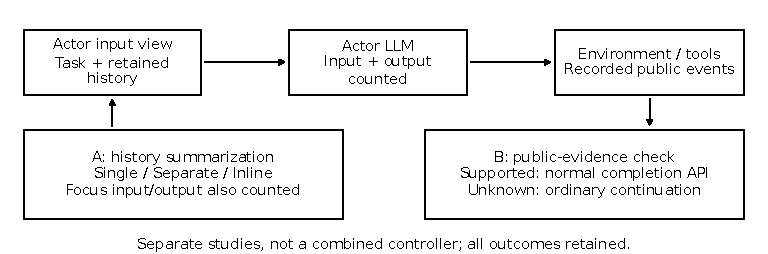
\includegraphics[width=130mm]{figures/control_points.pdf}
\caption{入力履歴と次の生成の要否を制御する二つの作用点．実験A，Bは別々に実行する．}
\ecaption{Two control points for input history and further generation, evaluated in separate studies.}
\label{fig:architecture}
\end{figure*}

\subsection{全呼出しを含む費用と最終成功}
条件$p$のモデル呼出し集合を$\mathcal C_p$とし，実際の入力$I_c$と出力$O_c$から
\begin{equation}
 T_p=\sum_{c\in\mathcal C_p}(I_c+O_c)
 \label{eq:cost}
\end{equation}
を求める．actorとfocus，不採用要約，失敗時の既知使用量も含め，cached inputを控除しない．論理トークン数は金銭課金や実行時間そのものではない\cite{xu2026tokenpilot}．圧縮役を含む費用評価はACON\cite{kang2026acon}にも存在し，会計方法自体を新規技術とはしない．局所的な入力削減と，生成全体の費用削減も区別する．

品質は，課題終了後の状態に対するAppWorld\cite{trivedi2024appworld}の公式評価器の成功・失敗で測る．評価の正解や詳細を実行中のモデルへ返さない．成功数の一致だけでなく，同じ課題の成功を失っていないかを確認する．不明使用量がある場合は既知小計と件数を残し，0へ補完しない．異なる実験の費用や課題数は合算しない．

\section{実験A：要約の呼出し配置}
\subsection{条件}
写真操作，精算，返金，CSV処理の既知4課題に対し，単発別要約（Single），別呼出し反復（Separate），同時反復（Inline）を各1回，計12条件実行した．全条件は同じMiniMax-M3（GGUF，IQ4\_XS），llama.cpp b11669，文脈長65,536を用いた．model seedの基点は57，world seedは42で，呼出しの役割・順序に従いseedを増分した．

要約機会の入力長閾値は16,384トークン，直近2ターンを保持し，反復では新規完了ターン3以上を要求する．単発の最大機会数は1，反復は3である．要約は合計8,192文字以下とし，次のactor入力全体が短くなる場合に採用する．単発と別呼出し反復はfocus出力上限4,096で，focus費用も式\eqref{eq:cost}へ含める．

各条件の上限は80モデル要求，450,000トークン，作業1,800秒で，環境APIは写真160，他3課題80要求とした．actor温度1.0，focus温度0.7，並列実行数1，KV cache q8\_0，計算機はApple M3 Ultra・メモリ256 GiBである．実装と全条件の記録を公開する\footnote{\url{https://github.com/sophiria1225/AI-}}．

\subsection{全4課題の結果}
表\ref{tab:summary}に全12条件の費用を示す．全方式が4/4成功し，使用量不明は0だった．SeparateはSingleより107,873トークン（12.07\%）少なかった．この差は全てCSVの440,461から332,588への減少であり，他3課題は同値である．要約採用回数も，CSVはSingleの1回に対して両反復方式が2回，写真は全方式1回，精算・返金は0回だった．したがって，全4課題で一様に改善した結果ではない．

InlineはSingleより6.34\%少なかったが，強いSeparate対照より51,266トークン（6.53\%）多かった．写真だけではInlineが10,497少ない一方，CSVではSeparateより61,763多く，この増加が上回った．専用要約呼出しを無くすことと，全仕事を安くすることは同義ではない．図\ref{fig:results}（a）はCSV以外の3課題とCSVを分けてこの内訳を示す．

\begin{table*}[t]
\caption{実験Aの全12条件の論理入出力．全セル公式成功，使用量不明0．}
\ecaption{Logical input/output for all 12 conditions in study A; all succeed with known usage.}
\label{tab:summary}
\centering
\begin{tabular}{lrrr}\hline
課題 & Single & Separate & Inline\\\hline
写真操作 & 139,871 & 139,871 & 129,374\\
精算 & 211,110 & 211,110 & 211,110\\
返金 & 102,087 & 102,087 & 102,087\\
CSV処理 & 440,461 & 332,588 & 394,351\\\hline
全4課題 & 893,529 & 785,656 & 836,922\\\hline
\end{tabular}
\end{table*}

\begin{table*}[t]
\caption{実験Bの全4観測．同じ写真1課題で，全観測公式成功，使用量不明0．}
\ecaption{All four observations in study B concern one photo task and succeed with known usage.}
\label{tab:termination}
\centering
\begin{tabular}{llrrr}\hline
Interface & 制御 & 論理入出力 & モデル呼出し & API要求\\\hline
文書取得必須 & 通常継続 & 130,439 & 15 & 104\\
 & 証拠付き終了 & 91,116 & 13 & 100\\
公開名アクセス & 通常継続 & 151,664 & 14 & 103\\
 & 証拠付き終了 & 112,233 & 12 & 99\\\hline
\end{tabular}
\end{table*}


\section{実験B：公開証拠に基づく終了}
\subsection{条件}
同じ既知写真課題について，API文書取得を必須とするinterfaceと，公開API名からのアクセスを許すinterfaceの2条件を比較した．各interfaceで，既に閉鎖した通常継続を対照に，同じ初期状態・モデル・seed・案内・予算から新たに終了制御を各1回実行した．seedの基点は42であり，実験Aとは別の履歴・設定である．同じMiniMax-M3 IQ4\_XSとllama.cpp b11669を用い，上限は80要求，450,000トークン，作業1,800秒，API160要求である．

制御は既知1要求文型の手書き検査である．完全な元集合，移動前の日時，公開時計，対象全件の移動先，名前保持などの公開根拠を検査する．支持が揃った最初の生成境界で，通常の完了通知を1回だけ送る．未知作用や不確定な集合を完了扱いにせず，未来の応答・正解を利用しない．判定，保存，通知を含む実行時間と，通知APIを計上する．

\subsection{成功を保った局所的な削減}
表\ref{tab:termination}と図\ref{fig:results}（b）に全4観測を示す．文書取得必須では130,439から91,116へ30.15\%，公開名アクセスでは151,664から112,233へ26.00\%減った．両対照・両制御とも公式成功，使用量不明0で，各条件2生成・4API要求が少なかった．完了通知は省かず，対象の移動後に続いていた4回の確認APIと，それに伴う生成を実行しなかった．

実行した公開API等の前半記録は対照と一致し，最終13データベースのhashも全て一致した．ただし，要求・モデル応答全文のstrict prefix一致は不成立であり，その事前基準を変更しない．手書きの既知要求文型による各1回の比較であって，平均因果効果や汎用の終了保証ではない．

\begin{figure*}[t]
\centering
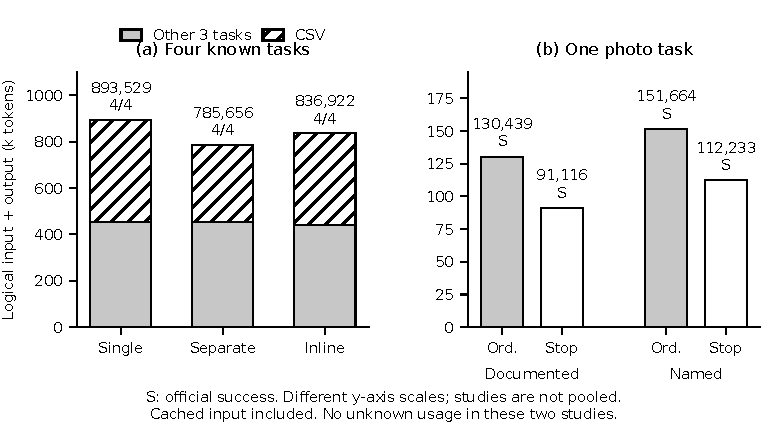
\includegraphics[width=130mm]{figures/separate_studies.pdf}
\caption{別々の実験における費用．（a）全4課題は各方式4/4成功，（b）同じ写真課題の全4観測は成功．二つの縦軸と集計範囲は異なる．}
\ecaption{Costs in separate studies. All conditions succeed; the axes and aggregation scopes differ.}
\label{fig:results}
\end{figure*}

\section{考察と限界}
二つの実験では，履歴再入力や完了後の継続を制御した既知条件で，成功を保った費用削減を観測した．一方，通常制御を複雑にすれば改善するとは限らない．InlineがSeparateに負けた比較は除外できない．後続のreceipt表示実験でも，一方のseedでは成功3/4から4/4かつ1.89\%減だったが，もう一方では成功を1件失い，両方式に使用量不明が残った．更に閾値8,192の再帰置換と差分保持の比較では，成功が3/4から2/4へ減り，使用量不明1件のため全体削減率は確定しなかった．これらを正例へ合算しない．

本稿は閉鎖済み開発実験から，正例と直接対照を事後に整理した評価である．既知課題，単一モデル量子化，少数のseedと反復，手書き完了規則に限定され，未見課題への独立確認ではない．12.07\%と26--30\%を同じ母集団の平均にせず，一般的な品質維持，統計的非劣性，新しい圧縮・終了原理の成立は主張しない．今後は具体的な候補と対照を固定して，適用範囲と失敗を含む全件を別に検証する必要がある．

\section{むすび}
通常のハーネス制御を全仕事の論理入出力と最終成功で評価した．既知4課題では別呼出し反復要約が単発より12.07\%少なく，別実験の既知写真課題2条件では証拠付き終了が26--30\%少なかった．同時要約が別呼出し反復より高費用だった対照も含め，専用要約呼出しの削減と全仕事の費用削減を区別した．既知条件での結果は，履歴更新と完了後継続の制御を最終成功と合わせて評価する必要性を示す．

% Verified official publication metadata; all authors retained.
% Bibliographic source URLs and detailed verification are in references.bib
% All seven references are formally published conference papers.
\begin{thebibliography}{9}
\bibitem{yao2023react}
S. Yao, J. Zhao, D. Yu, N. Du, I. Shafran, K. Narasimhan, and Y. Cao,
``ReAct: Synergizing reasoning and acting in language models,''
Proc. ICLR, May 2023.

\bibitem{wang2024codeact}
X. Wang, Y. Chen, L. Yuan, Y. Zhang, Y. Li, H. Peng, and H. Ji,
``Executable code actions elicit better LLM agents,''
Proc. ICML, PMLR, vol.235, pp.50208--50232, July 2024.

\bibitem{jiang2024longllmlingua}
H. Jiang, Q. Wu, X. Luo, D. Li, C.-Y. Lin, Y. Yang, and L. Qiu,
``LongLLMLingua: Accelerating and enhancing LLMs in long context scenarios via prompt compression,''
Proc. ACL, vol.1, pp.1658--1677, Aug. 2024.
doi: 10.18653/v1/2024.acl-long.91.

\bibitem{kang2026acon}
M. Kang, W.-N. Chen, D. Han, H. A. Inan, L. Wutschitz, Y. Chen,
R. Sim, and S. Rajmohan,
``ACON: Optimizing context compression for long-horizon LLM agents,''
Proc. ICML, PMLR, vol.306, pp.55321--55375, July 2026.

\bibitem{xu2026tokenpilot}
B. Xu, Z. Xue, D. Chen, C. Fu, C. Wu, C. Huang, C. Jiang, J. Fang,
X. Deng, Y. Chen, Y. Yao, X. Wang, J. Shang, H. Chen, and N. Zhang,
``TokenPilot: Cache-efficient context management for LLM agents,''
Findings of ACL: EMNLP 2026, pp.19034--19049, Oct. 2026.

\bibitem{lu2025runaway}
Q. Lu, L. Ding, S. Cao, X. Liu, K. Zhang, J. Zhang, and D. Tao,
``Runaway is ashamed, but helpful: On the early-exit behavior of large language model-based agents in embodied environments,''
Findings of ACL: EMNLP 2025, pp.24014--24027, Nov. 2025.
doi: 10.18653/v1/2025.findings-emnlp.1304.

\bibitem{trivedi2024appworld}
H. Trivedi, T. Khot, M. Hartmann, R. Manku, V. Dong, E. Li, S. Gupta,
A. Sabharwal, and N. Balasubramanian,
``AppWorld: A controllable world of apps and people for benchmarking interactive coding agents,''
Proc. ACL, vol.1, pp.16022--16076, Aug. 2024.
doi: 10.18653/v1/2024.acl-long.850.

\end{thebibliography}

\end{document}
